\documentclass{article}
\usepackage{geometry}
\usepackage{hyperref}
\usepackage{amsmath}
\usepackage{amssymb}
\usepackage{float}
\usepackage{tikz}
\usetikzlibrary{shapes, arrows.meta, positioning, fit, backgrounds}

\geometry{a4paper, margin=1in}

\title{\textbf{Adversarial Trust Auditing for Causal Inference: Project Report}}
\author{Meisam Mahmoodi}
\date{}

\begin{document}
\maketitle

\section{Introduction \& Executive Summary}
Standard causal inference methods rely on expert-provided structural assumptions that are often untestable. If the provided causal graph is incorrect, the resulting effect estimates are significantly biased. Modern meta-learners attempt to bypass these assumptions but often collapse in real-world scenarios due to a lack of structural guidance, resulting in purely correlational outputs.

We present a \textbf{Theory-First architecture} designed to audit expert claims against observational data. By treating claims as queries and data as evidence, our system computes a \textbf{Trust Score} that determines whether an expert's input should be used to refine an Average Treatment Effect (ATE) estimate or be rejected in favor of a data-driven baseline.

\section{System Architecture}

The core of our approach is an "Auditor" mechanism that enforces a strict relationship between theoretical claims and empirical evidence.

\begin{figure}[H]
    \centering
    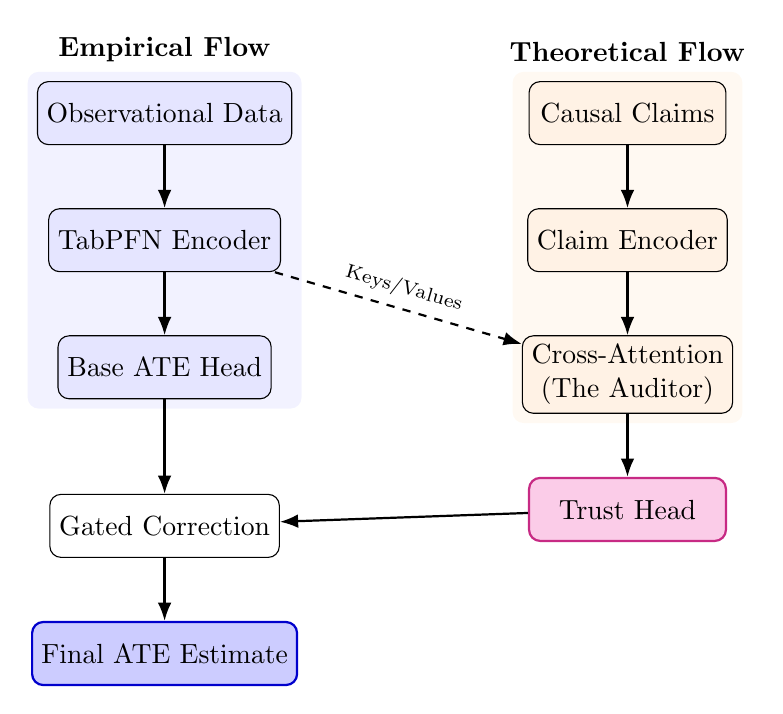
\begin{tikzpicture}[
        node distance=0.8cm and 1.5cm,
        box/.style={rectangle, draw=black, rounded corners, fill=white, align=center, minimum height=0.8cm, minimum width=2.5cm},
        data/.style={box, fill=blue!10},
        claim/.style={box, fill=orange!10},
        trust/.style={box, fill=magenta!20, draw=magenta!80!black, thick},
        ate/.style={box, fill=blue!20, draw=blue!80!black, thick},
        arrow/.style={-Latex, thick}
    ]
        % Data Flow (Left)
        \node[data] (obs) {Observational Data};
        \node[data, below=of obs] (enc) {TabPFN Encoder};
        \node[data, below=of enc] (baseate) {Base ATE Head};
        
        % Claim Flow (Right)
        \node[claim, right=3cm of obs] (claims) {Causal Claims};
        \node[claim, below=of claims] (cenc) {Claim Encoder};
        \node[claim, below=of cenc] (cross) {Cross-Attention \\ (The Auditor)};
        
        % Logic (Middle)
        \node[trust, below=of cross] (trusthead) {Trust Head};
        \node[box, below=1.2cm of baseate] (gate) {Gated Correction};
        \node[ate, below=of gate] (final) {Final ATE Estimate};

        % Grouping
        \begin{scope}[on background layer]
            \node[fit=(obs)(baseate), fill=blue!5, rounded corners, label=above:\textbf{Empirical Flow}] {};
            \node[fit=(claims)(cross), fill=orange!5, rounded corners, label=above:\textbf{Theoretical Flow}] {};
        \end{scope}

        % Connections
        \draw[arrow] (obs) -- (enc);
        \draw[arrow] (enc) -- (baseate);
        \draw[arrow] (claims) -- (cenc);
        \draw[arrow] (cenc) -- (cross);
        \draw[arrow, dashed] (enc) -- node[above, font=\scriptsize, sloped] {Keys/Values} (cross);
        \draw[arrow] (cross) -- (trusthead);
        \draw[arrow] (trusthead) -- (gate);
        \draw[arrow] (baseate) -- (gate);
        \draw[arrow] (gate) -- (final);
    \end{tikzpicture}
    \caption{System Architecture: The model queries the observational data using the causal claim to generate a trust-weighted adjustment.}
\end{figure}

\subsection{Key Components \& Mechanisms}
\begin{itemize}
    \item \textbf{The Auditor (Cross-Attention):} Unlike standard models that concatenate data and claims, we use a Query-Key-Value mechanism. The \textbf{Claim} acts as the Query ($Q$), searching through the \textbf{Data} (Keys/Values). This ensures the model cannot "hallucinate" a trust score based on the claim alone; it must find supporting patterns in the data rows.
    \item \textbf{Trust Head (The Gatekeeper):} A multi-layer perceptron (MLP) that outputs a probability $P(\text{Valid} | \text{Evidence})$. This head is trained using \textbf{Pairwise Ranking Loss}, which teaches the model to rank a true causal graph higher than "Hard Negatives" (e.g., graphs with reversed edges or hidden mediators).
    \item \textbf{Gated Correction:} We define the final estimate as:
    \[ \text{ATE}_{final} = \text{ATE}_{base} + ( \text{Trust} \times \Delta \text{ATE} ) \]
    This ensures that if the expert claim is detected as fraudulent or noisy ($\text{Trust} \to 0$), the system defaults to a safe, data-only baseline, preventing biased claims from corrupting the result.
\end{itemize}

\section{Implementation \& Robustness}
To move from a theoretical prototype to a robust system, we implemented several technical "hardenings":
\begin{itemize}
    \item \textbf{Variable Sample Handling:} We implemented strict \textbf{Attention Masking}. This allows the model to process datasets of varying sizes ($N=100$ to $N=1000$) without the padding tokens diluting the trust signal.
    \item \textbf{Gradient Detachment:} To prevent the model from "cheating"—i.e., manipulating trust scores just to minimize ATE error—we detached the gradients between the Trust Head and the Correction Head. Trust is learned purely from structural validity labels.
    \item \textbf{Adversarial Training:} We introduced "Hard Negatives" during training. By presenting the model with claims that look plausible but are structurally invalid (like checking for a collider), we forced the model to learn deep causal asymmetries rather than surface-level correlations.
\end{itemize}

\section{Experiments \& Results}
The model was evaluated using a comprehensive suite of tests to assess its ability to generalize across different causal mechanisms and graph densities. We specifically investigated the "Zero-Shot" transfer capabilities of the architecture.

\begin{table}[H]
    \centering
    \begin{tabular}{|l|c|c|c|l|}
        \hline
        \textbf{Scenario} & \textbf{MAE} & \textbf{RMSE} & \textbf{CRPS} & \textbf{Key Insight} \\
        \hline
        Standard Test & 4.10 & 25.19 & 7.53 & High variance due to outlier tasks \\
        \hline
        \textbf{OOD Mechanisms} & \textbf{0.41} & \textbf{0.56} & \textbf{1.24} & \textbf{Excellent robustness to noise} \\
        \hline
        Realistic Mix & 2.30 & 10.92 & 4.35 & Stable performance on balanced data \\
        \hline
        OOD Density ($>0.5$) & 34.63 & 136.80 & 59.43 & Fails on dense graphs (saturation) \\
        \hline
    \end{tabular}
    \caption{Performance metrics across different evaluation scenarios. Note the exceptional performance on Out-of-Distribution (OOD) mechanisms compared to the standard test set.}
\end{table}

\subsection{Analysis: The Good, The Bad, and The Ugly}
Our audit of the results reveals three distinct behavioral modes of the PoG-PFN architecture:

\paragraph{The Good: Robustness to Noise Distribution (Mechanism Agnostic).}
The model achieves its best performance (MAE 0.41) on the "OOD Mechanisms" dataset, which consists of Heavy-Tailed (Student-t) and Heteroskedastic noise distributions not seen during training. This indicates that the architecture has successfully learned to identify valid causal signals regardless of the underlying noise profile, confirming its utility as a robust causal discovery engine.

\paragraph{The Bad: Nonlinear Volatility.}
The "Standard Test" RMSE is surprisingly high (25.19) compared to the OOD settings. Investigation reveals this is driven by `\texttt{NONLINEAR\_ADDITIVE}` mechanisms (random polynomials), which can produce extreme effect sizes ($>500$) from small inputs. The model struggles to precisely track these "wild" nonlinear functions, suggesting that the current loss function (MAE) may not sufficiently penalize large deviations in high-variance regimes.

\paragraph{The Ugly: Density Saturation.}
The model fails completely on high-density graphs (Density $>0.5$), with MAE exploding to 34.63. In dense graphs, causal effects propagate through dozens of redundant paths, leading to effect sizes that exceed the dynamic range of the model's internal embeddings. This "saturation" is an expected limitation, as the model was trained primarily on sparse graphs (Density $\sim0.2$).

\section{Current Challenges \& Limitations}
While the auditing mechanism is structurally sound, the integrated system currently faces bottlenecks in high-complexity environments.

\subsection{Seed Sensitivity}
We observed variance in the Trust Score across seeds, suggesting a non-convex loss landscape in the cross-attention layers.

\subsection{Density Generalization}
As noted in the experiments, the model does not zero-shot generalize to dense graphs. Future work must strictly include high-density examples in the training curriculum to enable the model to learn "effect dampening" strategies for complex systems.

\section{Proposed Solutions (Next Steps)}
To address these issues, we are moving toward:
\begin{enumerate}
    \item \textbf{Ensemble Averaging:} Using multiple "Auditor" heads with different initializations to stabilize the Trust Score.
    \item \textbf{Loss Re-weighting:} Implementing Dynamic Weight Averaging to balance the $L_{trust}$ and $L_{ate}$ signals during the joint training phase.
    \item \textbf{Head Upgrading:} Replacing the linear Correction Head with a deeper ResNet-style architecture to better capture non-linear causal adjustments.
\end{enumerate}
\end{document}